\section{Cupper}
\label{sec:cupper}

No contexto de DevOps, automação e infraestrutura como código, a ferramenta
proposta por este trabalho, Cupper, propõe auxiliar na extração de configuração
de um ambiente incluso em uma infraestrutura. As configurações extraídas são
transformadas em código em padrões da receita Chef (Figura \ref{fig:cupper_geral}).

\begin{figure}[h]
  \label{fig:cupper_geral}
  \centering
  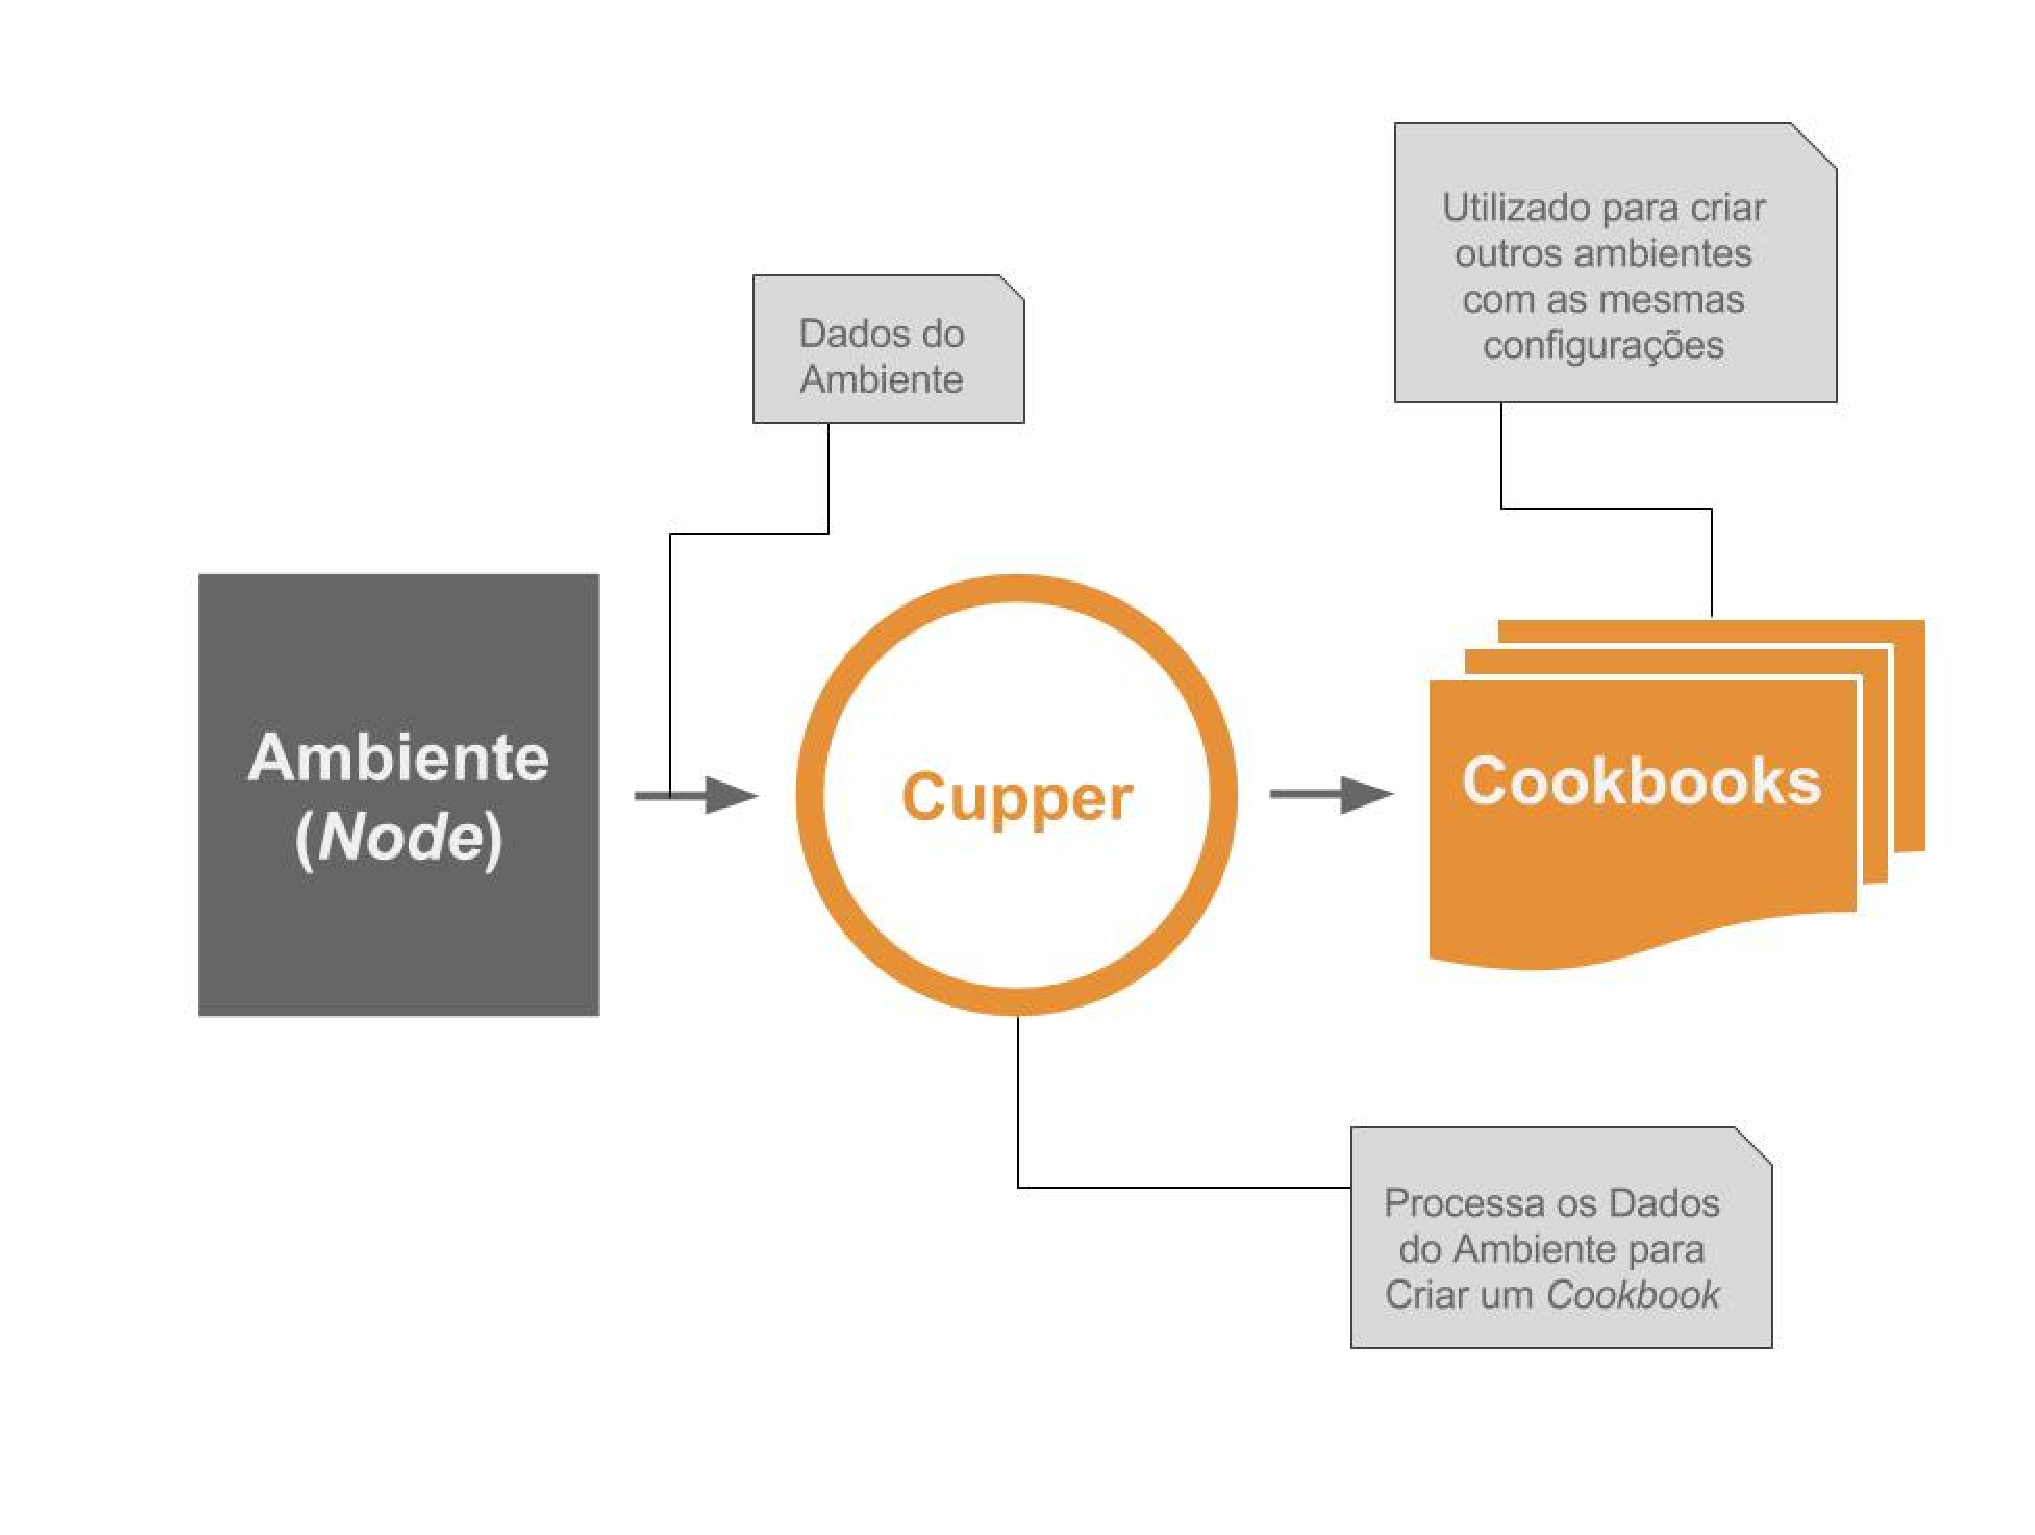
\includegraphics[width=0.8\textwidth]{figuras/cupper_geral.eps}
  \caption{Cupper - Visão geral}
\end{figure}

%TODO: Incluir pontos importantes para o entendimento geral do Cupper
%   incluir os concorrentes?
O detalhamento do Cupper será abordado no capítulo~\ref{chap:espec}.
